\section{Auditory-Model-Based Method}
\label{sec:methods:auditory}

As shown in Figure \ref{fig:fig3}, the auditory-model-based method for ensemble width estimation consists of two main components: a binaural auditory model that extracts features from the input signals, followed by a gradient-boosted decision tree regressor that predicts the ensemble width \cite{antoniuk_ensemble_2024}. The auditory model processes the binaural signals through a gammatone filterbank and extracts standard binaural cues, including interaural time differences (ITD), interaural level differences (ILD), and interaural cross-correlation (IACC).

\begin{figure}[htbp]
	\begin{center}
		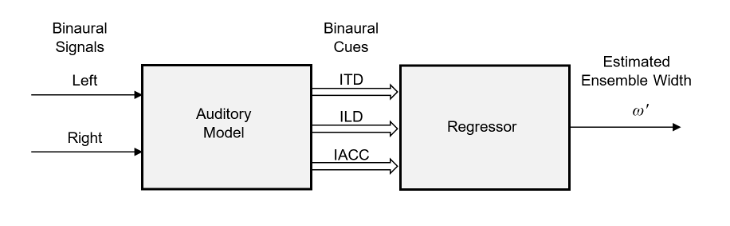
\includegraphics[width=1.0\linewidth]{img/auditory_flowchart.png} 
	\end{center}
	\caption{A flowchart of the auditory-model-based method \cite{antoniuk_ensemble_2024}} \label{fig:fig3}
\end{figure}

The auditory model is based on the work of S{\o}ndergaard and Majdak~\cite{blauert_technology_2013}, enhanced by May et al.~\cite{may_probabilistic_2011}, and further refined by Decorsi{\`e}re and May~\cite{decorsiere_auditory_2016} within Two!Ears Project~\cite{raake_computational_2016}. The~model consists of a gammatone filterbank with 64 frequency channels spanning from 100~Hz to 16~kHz. For each frequency channel, the inner hair-cell envelopes are extracted through half-wave rectification followed by low-pass filtering using a second-order Butterworth filter with a~1~kHz cutoff frequency. This simulates the loss of phase-locking in the~auditory nerve at higher frequencies. Rate maps, representing auditory nerve firing rates, are then calculated by smoothing the inner hair-cell signal with a~leaky integrator (time constant of 8~ms) and averaging within 20~ms Hann-windowed frames with 10~ms step size. Finally, the rate maps were used to estimate the binaural cues.

The features extracted in the~previous component are aggregated across time-frames by computing their mean values and standard deviations, resulting in a total of 384 feature vectors (64 frequency channels $\times$ 3 types of cues $\times$ 2 statistics). These aggregated features are then used as input to the~regressor, whose objective is to estimate the ensemble width of the binaural audio signal. The~regressor employs gradient-boosted decision trees implemented with LightGBM, known for its computational efficiency and accuracy \cite{ke_lightgbm_2017}. The~model's hyperparameters---including the number of leaves, tree depth, and learning rate---were optimized using grid search procedure. The final training was conducted using validation set and early-stopping technique based on mean absolute error. For further details, see~\cite{antoniuk_ensemble_2024}.
